% Chapter X

\chapter{Results} % Chapter title
\label{ch:results} % For referencing the chapter elsewhere, use \autoref{ch:name} 

This chapter is dedicated to the description of the OCT software that was developed for this thesis. This application handles the data acquisition task, controls the galvanometric system and performs real-time processing and visualization of the acquired OCT data. \\

\noindent The transversal resolution of the system described in \autoref{ch:setup} is also evaluated using the test resolution target introduced in the same chapter. \\

\noindent Finally, a series of B-scans, C-scans and \emph{en-face} images of a variety of different samples is presented. A subset of these images were acquired using a second SS-OCT system designed to work in the 1060 nm range. 


%----------------------------------------------------------------------------------------

\section{Data Acquisition Software}

The final component that is needed to obtain a working SS-OCT system is a computer application that handles data acquisition and image visualization. This program should be able to achieve real-time performances, enabling a low-delay video stream of cross-sectional OCT data. Ideally, the total acquisition rate of the system in terms of B-scans per second should be limited by the scanning speed of the galvanometric mirrors and not by the OCT software. In fact, given the transversal resolution of the system, the FOV of the scanning lens and the spot size on the focal plane, there exists a maximum frequency at which the mirrors can be driven in order to obtain distortion-free images. An extensive analysis on this matter is carried out in \cite{Calabrese2017}. \\


%Leave this chapter for the explanation of the software, technologies used, performance achieved and showcase of the measurements. B-scans, volumes and enface. Also include control of the galvo mirrors in here since it's about C++ programming. 

%Explain in detail the fact that for real time the average time to process has to be < frame time and explain buffer ring to get buffer from board using DMA. Check datasheet in the pdfviwer since there is a nice explanation of async drivers. 

\noindent The application has been developed for the Windows 10 Operating System using the Object-Oriented C++ programming language, which is the only one that allows low-level memory management among those supported by the ATS9350 acquisition board. Additionally, it permits the native integration of the high performance graphics library called OpenGL\footnote{\url{https://www.opengl.org/}}. \\


The code is built using the Qt application framework\footnote{\url{https://www.qt.io/}}, which consists in a set of tools for event handling and the design of \acp{GUI}. In Qt, asynchronous code can be easily written using the Signals and Slots paradigm: when a particular event occurs, an object \emph{emits} a signal; objects that are connected to this signal will execute the appropriate slot, which is a function that takes the parameters passed by the connected signals and perform some actions. For example, the object dealing with OCT data acquisition can emit a signal with a newly acquire B-scan, while a data visualization object connected to this signal can retrieve this data and display it without blocking the acquisition task. 

\begin{figure}[htb]
	\myfloatalign
	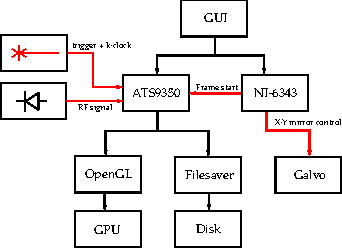
\includegraphics[width=0.6\linewidth]{gfx/ch4/dataflow}
	\caption{Data flow of the OCT application.}\label{fig:dataflow}
\end{figure}

The data flow of the application in illustrated in \autoref{fig:dataflow}. The \ac{GUI} initiates an acquisition by communicating with the ATS9350 board and an additional \ac{DAQ} board dedicated to the control of the galvo mirrors and to supply a "frame start" signal. This device is the National Instruments USB-6343\footnote{\url{http://www.ni.com/it-it/support/model.usb-6343.html}}, which is a USB board equipped with 4 analog outputs, 32 analog inputs and 48 digital I/O ports capable of 900 kilosamples/s. Once the ATS9350 receives the "frame start" signal, it will listen for A-scan triggers provided by the Axsun laser and start sampling the interference signal using the $k$-clock. After the acquisition of a B-scan is complete, the board returns a memory block containing the acquired data to the application, that will then process it and send it to two objects which asynchronously display it using OpenGL and save it to disk. 

\subsection{Controlling the galvanometric mirrors}
In order to control the galvo system, voltage signals that are proportional to the scan angle have to be sent to its driver boards. As explained in \autoref{ch:setup}, two separate signals are needed for each mirror: one for positive and one for negative angles. This requires the use of a \ac{DAQ} board with at least 4 analog output ports, explaining the choice of the USB-6434. 

To scan an area of the sample, the $X$ motor is driven with a triangle wave of frequency $f_b$ while the $Y$ motor is controlled with a "staircase" signal with a number of "steps" equal to the number of frames in the volume. At the start of each rising edge of the triangle wave, a TTL pulse will also be generated and sent to the AUX port of the ATS9350 board to signal the start of a B-scan. An example is available in \autoref{fig:galvo-signals}, where the B-scan frequency is $f_b = 20$ Hz, and the number of frames per volume is equal to 4. Using these voltages, the area that will be scanned is equal to 

\begin{equation}
	\mathcal{A} = \left[2\cdot EFL \tan\left( 2 \times 2 V \times 1  ^ \circ/V \times \frac{\pi}{180}\right)\right]^2 \approx 7.55\times 7.55 \text{ mm}^2,
\end{equation}
where $EFL = 54$ mm is the effective focal length of the lens introduced in \autoref{ch:setup}. 
If only cross-sectional images are required, the $Y$ motor will be controlled with a constant voltage. 

During the falling edge of the triangle wave the $X$ mirror will return to its initial position, meaning that the data generated in this time interval is not useful. Hence, the number of A-scans to acquire in order to scan the entire space covered by this mirror is

\begin{equation}\label{eq:bscan-maxwidth}
	N = \frac{1}{2} \frac{f_a}{f_b},
\end{equation}
where $f_a = 100$ kHz is the sweep repetition rate of the laser. 

\begin{figure}[htb]
	\myfloatalign
	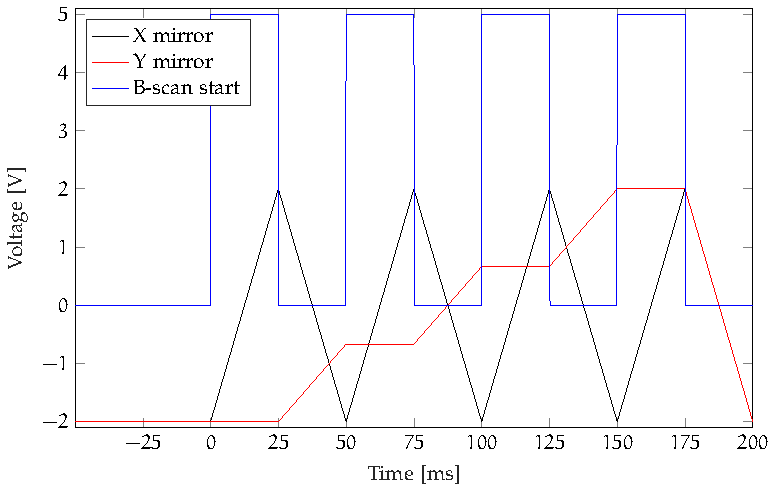
\includegraphics[width=0.9\linewidth]{gfx/ch4/galvo-signals}
	\caption{Signals used to control the galvanometric mirrors.}\label{fig:galvo-signals}
\end{figure}

Recalling that the each signal must be split in its positive and negative parts as in \autoref{eq:galvo-split-signals}, the actual signals that will be sent to the galvo driver boards will look like those in \autoref{fig:galvo-signals}.

\begin{figure}[htb]
	\myfloatalign
	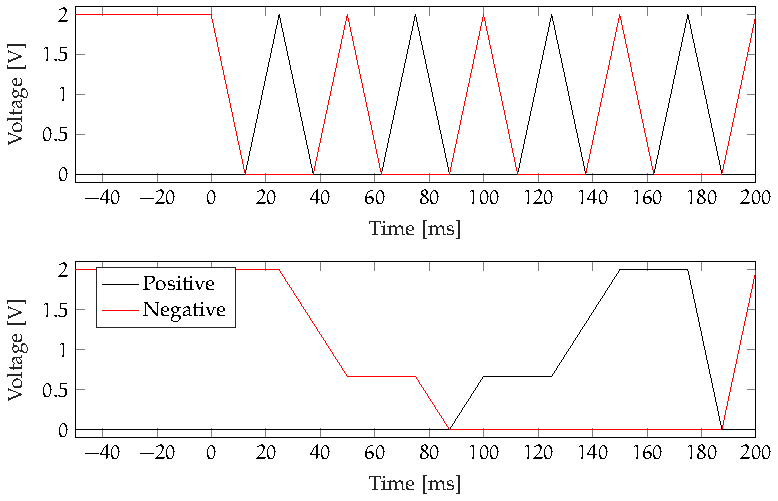
\includegraphics[width=0.9\linewidth]{gfx/ch4/galvo-signals-split}
	\caption{Signals used to control the galvanometric mirrors.}\label{fig:galvo-signals-split}
\end{figure}

\subsubsection*{Configuring the NI-6343 board}
The control of the USB-6343 board is integrated in the OCT application using the DAQmx drivers developed by National Instruments. The program is organized in \emph{tasks}; each task is a collection of channels which corresponds to a measurement or generation to perform and that can be configured independently to other tasks, specifying triggering, timing and other properties. 

In our case two tasks are created:
\begin{enumerate}
	\item Digital Task: handles the generation of the "Frame start" signal. It consists in a single digital channel which can be configured as a "digital pulse" with the \texttt{DAQmxCreateCOPulseChanFreq} function, specifying the output port of the board, the frequency of the pulse and its duty cycle. In order to generate a sequence of pulses instead of just a single one, the function \texttt{DAQmxCfgImplicit\-Timing} must be called to configure the task as "continuous generation". 


	
	\item Analog Task: drives the galvo system with the aforementioned signals. This task is a collection of four analog channels, which can be added with the \texttt{DAQmxCreateAOVoltageChan} command, specifying the output ports and a maximum expected voltage. 
	
	The signals are computed and stored in an array of floating point samples which will be uploaded to a buffer on the board and converted into a continuous signal by a \ac{DAC}. The length of each signal is determined by the selected generation rate $R_{clk}$, the B-scan rate $f_B$ and the number of frames per volume $N_v$ as 
	\begin{equation}
		N_{\text{samples}} = R_{clk} \cdot \frac{1}{f_B} \cdot N_v,
	\end{equation}
	meaning that the buffer uploaded to the board has length $4 \cdot N_{\text{samples}}$, as two analog signals are required for each mirror. Just like before, "continuous generation" must be configured, otherwise a single volume (or a single frame in case of 2D acquisition) will be scanned. To synchronize the two tasks, analog data generation is triggered by the digital pulse train created above using the \texttt{DAQmxCfgDigEdgeStartTrig} function. 
		
\end{enumerate}


\subsection{Programming the ATS9350}
In \autoref{ch:setup}, the different acquisition modes supported by the ATS9350 board were introduced. In particular, for OCT applications No-Pre-Trigger AutoDMA must be used, as it is the only method which supports high trigger repeat rates. 

Data is organized in records and buffers: records correspond to a series of samples acquired for each trigger event, while buffers are a collection of 1 or more records. In OCT, records correspond to A-scans while buffers contain a complete B-scan. 

The data transfer between the board and the software works as follows:
\begin{enumerate}
	\item A list of data buffers are allocated on the PC and assigned to the board

	\item The board will acquire the number of records necessary to fill a buffer into its main memory. 

	\item Once the records have been acquired, an AutoDMA transfer will start copying the records from the on-board memory to the application buffer. At the same time, the board is acquiring new records to fill the next buffer, so no trigger events are missed while copying data to the PC.

	\item After the DMA transfer is complete, the board generates an interrupt, causing an event message to be sent to the application so it can start consuming data. 
	
	\item Once the buffer has been processed by the application, it must be returned to the board. The processing time must be sufficiently low so that the board will always have one buffer available, otherwise the acquisition will fail with a \emph{buffer overflow} error.
\end{enumerate}


\subsubsection{Triggering and Clocking}
Using the C++ library and headers supplied by AlazarTech, the board can be integrated in the OCT application and configured as needed. To start the acquisition of a B-scan, the AUX connector of the board is configured as "Trigger Enable In", meaning that every time a positive edge is detected on this connector the board will begin capturing a set amount of A-scans. This can be done with the following command:

\begin{lstlisting}[language=C,frame=tb]
AlazarConfigureAuxIO(boardHandle, AUX_IN_TRIGGER_ENABLE, TRIGGER_SLOPE_POSITIVE);
\end{lstlisting}

To trigger the acquisition of an A-scan instead, the sweep trigger provided by the laser is connected to the external trigger port. The board provides an advanced triggering system with two separate trigger engines, called J and K, that can either be used independently or combined to generate complex trigger events. In our case, engine K is disabled and engine J is configured to generate a trigger event when the signal connected to the external port reaches $V_{trig} = 0.71$ V. This value is passed to the board as an 8-bit integer code, calculated as 
\begin{align}
	\text{trigger code} &= 128 + 127 \times \frac{\text{trigger voltage}}{\text{input range}}\\
					&= 128 + 127 \times \frac{0.71}{5} = 146.
\end{align}

\begin{lstlisting}[language=C,frame=tb]

AlazarSetTriggerOperation(
	boardHandle,
	TRIG_ENGINE_OP_J,
	TRIG_ENGINE_J,
	TRIG_EXTERNAL,
	TRIGGER_SLOPE_POSITIVE,
	triggerCode, 
	TRIG_ENGINE_K, 
	TRIG_DISABLE, 
	TRIGGER_SLOPE_POSITIVE,
	128);

\end{lstlisting}

Similarly, clocking the board with the $k$-clock is achieved by using the \texttt{AlazarSetCaptureClock} function to select the clock source and the \texttt{AlazarSetExternalClockLevel} function to select the voltage level at which samples are captured.


\subsubsection{FFT module configuration}
Achieving real-time performance without the use of \ac{GPGPU} is possible only with the use of the onboard FPGA module that computes the FFT of acquired records. To configure this module, the following code snippet is used
\begin{lstlisting}[language=C,frame=tb]
AlazarFFTSetup(	fftHandle,
	CHANNEL_A,
	samplesPerAscan,
	fftLength,
	FFT_OUTPUT_FORMAT_U16_LOG,
	fftFooter,
	0,
	&bytesPerOutputRecord
);
\end{lstlisting}
where 

\begin{itemize}
	\item \texttt{CHANNEL\_A} is the channel used for data acquisition,
	\item  \texttt{samplesPerAscan} = 1536 is the number of useful sampling clocks of the $k$-clock (\autoref{tab:axsun-datasheet}).
	\item \texttt{fftLength} = 2048 is the length of the computed FFT.
	\item \texttt{FFT\_OUTPUT\_FORMAT\_U16\_LOG} is the format in which FFT data is returned to the application, meaning that an FFT sample is computed in logarithmic scale and stored in an unsigned 16-bit integer.
	\item \texttt{bytesPerOutputRecord} is the size of an FFT record, which in this case is equal to 2 $\times$ \texttt{fftLength} = 4096 bytes.
\end{itemize}

This means that setting a B-scan frequency $f_b$, the size of a buffer is given by
\begin{equation}\label{eq:bytesperbuffer}
	\texttt{bytesPerBuffer} = \frac{1}{2} \frac{f_a}{f_b} \cdot 4096 \text{ bytes},
\end{equation}
which for $f_b = 20$ Hz is equal to 10.24 Megabytes, corresponding to $2500$ A-scans per B-scan.\\

Additionally, the FFT module can be configured to zero-pad and multiply time domain records by a windowing function:
\begin{lstlisting}[language=C,frame=tb]
AlazarDSPGenerateWindowFunction(
	windowType, // type of window to generate
	window, // memory to store window
	samplesPerAscan, // length of the fft input
	fftLength - samplesPerAscan	// zero-padding
);

AlazarFFTSetWindowFunction(
	fftHandle,
	fftLength,
	window,
	NULL // reserved 
);
\end{lstlisting}

\subsubsection{The acquisition loop}\label{sub:acq-loop}
After determining the width of each B-scan, and consequently the buffer size, a list of buffers has to be allocated on the PC and posted to the board to be used for AutoDMA transfers. 

\begin{lstlisting}[language=C,frame=tb]
for (unsigned int i = 0; i < bufferCount; i++)
{
   U16 *buffer = (U16*)VirtualAlloc(NULL, bytesPerBuffer, MEM_COMMIT, PAGE_READWRITE);
   AlazarPostAsyncBuffer(boardHandle, buffer, bytesPerBuffer);
}
\end{lstlisting}

The application will wait for the board to fill these buffers with a B-scan by using the \texttt{AlazarDSPGetBuffer} function, which returns when a DMA transfer has completed. Once this happens, the B-scan will be converted to floating point values, copied to a new buffer to be stored on disk, and then converted to suitable format to be uploaded to the GPU and be visualized on screen. After these operations are completed, the buffer is returned to the board. 

In order to keep the GUI responsive, the following loop has to be run on a separate thread:

\begin{lstlisting}[language=C,frame=tb]
unsigned int acquiredBuffers = 0;
while (acquiredBuffers < totalBscans)
{
   int bufferIndex = acquiredBuffers % bufferCount;
   U16* buffer = bufferArray[bufferIndex];
	
   // wait for the buffer to be filled
   AlazarDSPGetBuffer(boardHandle, buffer, timeout)

   // process B-scan
   float *floatBscan = convertToFloat(buffer);
   byte *Bscan = convertToImage(floatBscan);
   
   emit saveToDisk(floatBscan);
   emit uploadToGPU(Bscan);
   
   // return buffer to the board
   AlazarPostAsyncBuffer(boardHandle, buffer, bytesPerBuffer)
}
\end{lstlisting}

To remove the complex conjugate artifacts introduced in \autoref{ch:theory}, half of the data points are dropped, reducing the number of samples of each B-scan to 
\begin{equation}
	N_{\text{samples}}^{\text{B-scan}} = \frac{1}{2} \frac{f_a}{f_b} \cdot 1024
\end{equation}

B-scans are processed using a multi-processing approach enabled by the OpenMP\footnote{\url{http://www.openmp.org/}} \ac{API}, reducing the processing time needed and minimizing the total delay. \\

The floating point values from which the image is computed are first clipped in an interval $[I_{min}, I_{max}]$ controlled through the \ac{GUI} and then mapped to a 1-byte integer with values in $[0, 255]$, enabling the user to filter out the noise floor and improve the contrast of the image. 
\begin{lstlisting}[language=C,frame=tb]
...
   if (sample > Imax)
     sample = Imax;
   if (sample < Imin)
     sample = Imin;
   float range = Imax-Imin;
   byte pixelValue = 255*(sample - Imin)/range;
...
\end{lstlisting}

Finally, the raw floating point data are sent to an object that asynchronously saves it to disk, while the computed image is displayed with OpenGL. 

\subsection{Processing time and delay}
Real-time data acquisition and visualization is achieved if the mean processing time of a B-scan is smaller than the time between two consecutive "frame start" signals:
\begin{equation}\label{eq:processing-limit}
	\mathbb{E}[T_p] < T_b = \frac{1}{f_b}.
\end{equation}
If this inequality is not respected the delay will grow indefinitely, regardless of the amount of buffers posted to the board. In fact, if $T_p$ is constant and smaller than $T_b$, two buffers would be sufficient, but given that the processing time is a stochastic process, allocating more buffers can prevent the board from overflowing due to external factors temporarily slowing down the processing speed, like processes with higher priority in non-real time Operating Systems. 

The average processing times were measured varying the B-scan frequency $f_b$ and the number of CPU cores used in the acquisition loop, acquiring 1000 B-scans for each scenario. As can be observed in \autoref{fig:processing-time}, the application can comfortably sustain the processing load for the entire range of framerates that was tested using just a single core. 

\begin{figure}[htb]
	\myfloatalign
	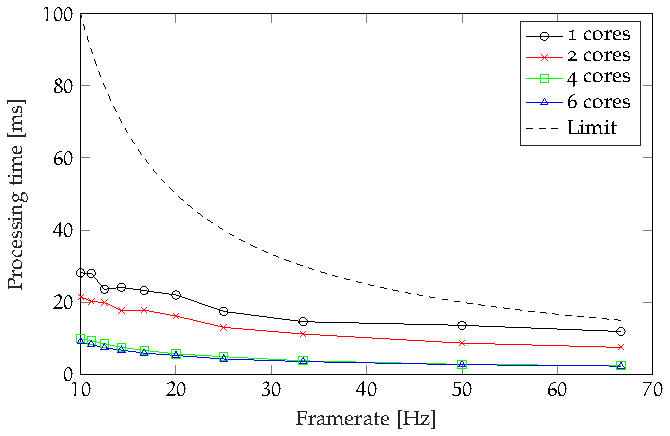
\includegraphics[width=0.8\linewidth]{gfx/ch4/processing-time}
	\caption{Processing time at different framerates and varying the number of CPU cores utilized.}\label{fig:processing-time}
\end{figure}

Even though a single core is enough to satisfy \autoref{eq:processing-limit}, using two or more is useful to reduce the total delay between the end of the acquisition of the B-scan and its visualization. This delay is computed as 
\begin{equation}
T_{\text{delay}} = T_{\text{DMA}} + T_p + T_{\text{GPU}},
\end{equation}
where $T_{\text{DMA}}$ is the time to transfer a B-scan from the ATS9350 to the application and $T_{\text{GPU}}$ is the time needed to upload the final image to the GPU and display it. Using \autoref{fig:gpu-throughput}, the DMA transfer time is computed as 

\begin{equation}
	T_{\text{DMA}} = \frac{\text{bytes per DMA buffer}}{\text{PCIe 2.0 throughput}} = \frac{\frac{1}{2}\frac{f_a}{f_b}\times 4096}{1.735 \text{ GB/s}},
\end{equation} 

where the PCIe throughput was measured in \autoref{sec:daq} using the AlazarDSO software. $T_{\text{GPU}}$ was instead measured directly inside the application. The result is visible in \autoref{fig:delay}: using 4 cores, delays lower
than 10 milliseconds are achievable even for large B-scans. 


\begin{figure}[htb]
	\myfloatalign
	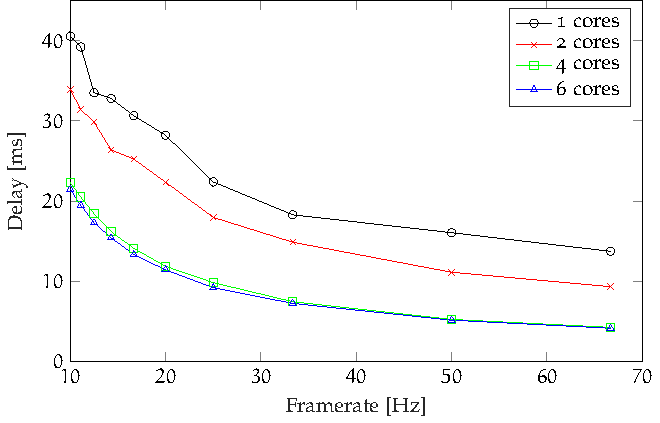
\includegraphics[width=0.8\linewidth]{gfx/ch4/delay}
	\caption{Total delay due to DMA transfer, CPU processing and GPU upload time.}\label{fig:delay}
\end{figure}

Finally, the GPU throughput is estimated as 
\begin{equation}
\eta_{\text{GPU}} = \frac{\text{bytes per image}}{\text{image upload time}} = \frac{\frac{1}{2}\frac{f_a}{f_b} \times 1024}{T_{\text{GPU}}},
\end{equation}
and illustrated in \autoref{fig:gpu-throughput}. The maximum throughput achieved by OpenGL is $\approx 9.8$ GB/s at 50 frames per second, corresponding to an image size of 1.024 MB. For lower framerates, and hence for bigger image sizes, the throughput decreases down to $7.7$ GB/s, which is about half the  maximum theoretical throughput supported by the PCIe 3.0 bus. 
\begin{figure}[htb]
	\myfloatalign
	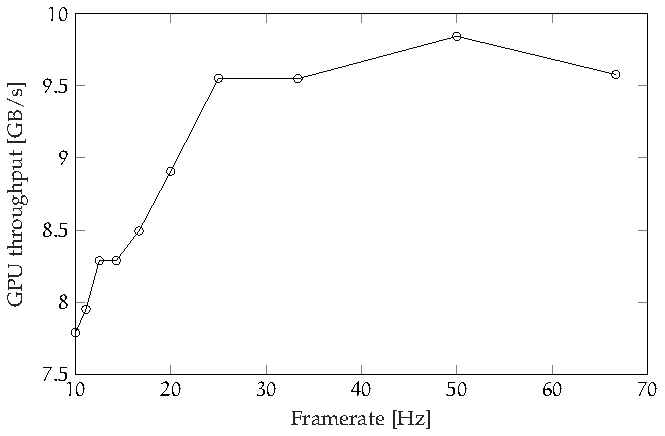
\includegraphics[width=0.8\linewidth]{gfx/ch4/gpu-throughput}
	\caption{GPU throughput using OpenGL.}\label{fig:gpu-throughput}
\end{figure}


\subsection{Saving data to disk}
A desirable feature for a OCT software is the ability to save the acquired data to disk so that further post-processing can be performed. In \autoref{sub:acq-loop} it was explained that each buffer returned by the board to the user application is duplicated, converted to floating point format and emitted using a Qt signal. A filesaving object connects to this signal and appends the received buffer to a dynamic FIFO queue. This structure is then emptied in an asynchronous loop running on a separate thread, writing each buffer to file in a binary format using standard C++ I/O operations. If the writing speed is not sufficiently high, the buffer fills up until the amount of \ac{RAM} available on the workstation is completely used or the acquisition stops. 

Considering that the size of each buffer is

\begin{equation}
	S = \frac{1}{2} \frac{f_a}{f_b} \times 1024 \times 4 \text{ bytes},
\end{equation}

the queue fills up at a rate of
\begin{equation}
\eta_{q} = S \cdot f_b = f_a \times 2048\text{ bytes/s} = 204.8\text{ Megabytes/s},
\end{equation}
meaning that a \ac{SSD} is needed for long acquisitions as regular \acp{HDD} usually do not exceed write speeds of $\sim 150$ MB/s. In fact, the write speed of the HDD installed in the OCT workstation was benchmarked with the AlazarDSO software, resulting in $141.3$ MB/s while the SSD averaged $348.7$ MB/s. 

\subsubsection{The SSD write cliff}
Even though this value is higher than $\eta_q$, for long acquisition sessions (tens of Gigabytes of data), the write speed of the SSD drops significantly, the queue fills up and the application exhibits lags and unresponsiveness. This behaviour is due to the \emph{SSD write cliff}. In flash-based SSDs, the memory consists in a number of blocks, each of which contains a number of pages. Blocks are the smallest erasable units whereas pages are the smallest writable units. After an SSD is filled with data, unused pages must be erased before new data is written. Since a block is the smallest erasable unit, in order to erase the unused pages the SSD must erase all pages on the block, regardless if they are active or unused. This means that active pages must be rewritten into another block with free cells. Writing a single page can result in multiple corresponding re-write operations, which can then trigger additional erase operations, causing a \emph{write amplification}\footnote{\url{http://crestingwave.com/sites/default/files/collateral/velobit_whitepaper_ssdperformancetips.pdf}}. 

\begin{figure}[htb]
	\myfloatalign
	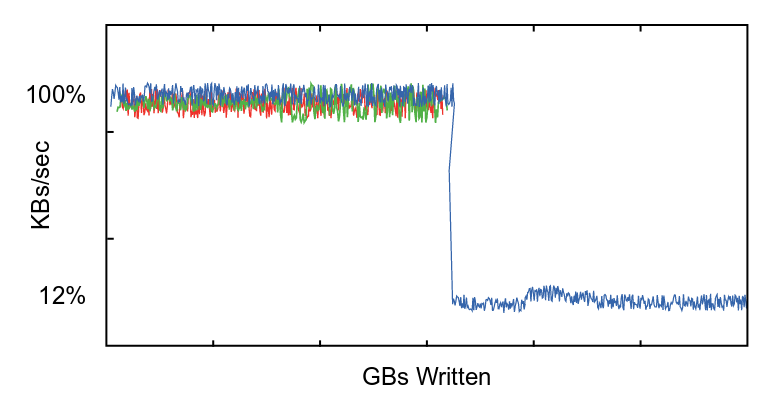
\includegraphics[width=0.8\linewidth]{gfx/ch4/write-cliff}
	\caption{The SSD write cliff.}\label{fig:write-cliff}
\end{figure}

Solutions to mitigate this effect could not be investigated in detail and will be addressed in future works. 

\clearpage
\section{Acquisitions}
In this section, a series of acquisitions made with the SS-OCT system described in the previous chapters are showcased.
\subsection{B-scans}
The first sample is the Thorlabs test target introduced in \autoref{sub:thickness-measurements}. In \autoref{fig:target-bscan} we can see the highly reflective chrome coating on the top, while the bottom surface is only visible where the clear pattern is present.
\begin{figure}[hbt]
	\centering
	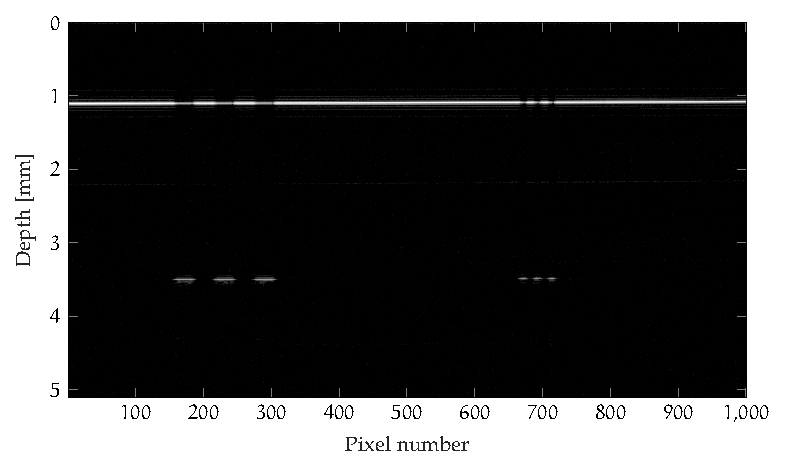
\includegraphics[width=0.8\linewidth]{gfx/ch4/axsun/target-bscan}
	\caption{B-scan of the Thorlabs test target.}\label{fig:target-bscan}
\end{figure}%----------


As explained in \autoref{sub:thickness-measurements}, the BPD utilized up until now does not amplify the received signal, meaning that the scattering generated by the analyzed samples could not be detected. To solve this issue, the BPD was replaced with another photodiode available in our laboratory, the Exalos EBR370010-02\footnote{\url{http://www.exalos.com/balanced-receivers/}}, which is equipped with a 50 dB transimpedance amplifier. A few comments have to be made in this regard:
\begin{itemize}
	\item Even though this receiver is designed to work in the 900-1200 nm range, acquisitions in the 1300 nm window were still possible. 
	
	\item The nominal bandwidth of 100 MHz will theoretically limit the imaging depth of the system, but in practice this effect was not appreciable. 
	
	\item The saturation power of $-13$ dBm required a slight adjustment of the reference arm: the collimator was misaligned until the received power was sufficiently low. 
\end{itemize}

The use of this receiver enabled the imaging of a lot of different samples. In \autoref{fig:bscans-artifacts} a few are presented:
\begin{itemize}
	\item Scotch tape (\autoref{fig:tape-bande}): the various layers of tape are clearly distinguishable. Each layer is measured at $\sim 60$ $\mu$m of thickness using $n=1$. 
		\item A fiber optic ribbon cable consisting of 12 \acp{SMF} (\autoref{fig:nastro-bande}).
		
	\item A dry orange peel (\autoref{fig:dry-orange-peel-bande}). 
	
	
\end{itemize} 

\begin{figure}[bth]
	\myfloatalign
	\subfloat[Scotch tape.]
	{\label{fig:tape-bande}
		\includegraphics[width=0.75\linewidth]{gfx/ch4/axsun/bande/tape}}\\
	\subfloat[Fiber optic ribbon cable.]
	{\label{fig:nastro-bande}
		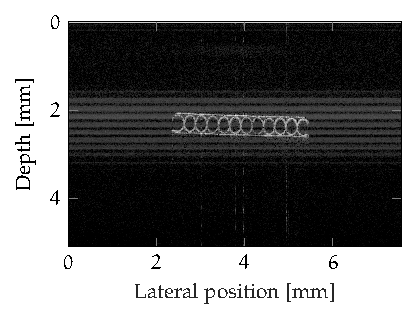
\includegraphics[width=.45\linewidth]{gfx/ch4/axsun/bande/nastro}} \quad
	\subfloat[Dry orange peel.]
	{\label{fig:dry-orange-peel-bande}
		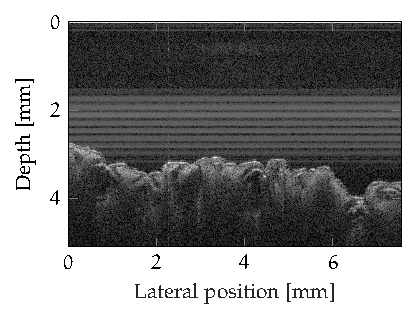
\includegraphics[width=.45\linewidth]{gfx/ch4/axsun/bande/dry-orange-peel}}
	\caption{B-scans of various samples afflicted by striped artifacts.}\label{fig:bscans-artifacts}
\end{figure}


%\begin{figure}[htb]
%	\centering
%	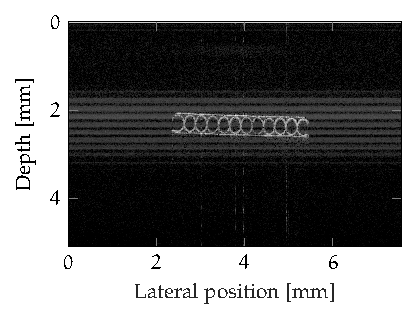
\includegraphics[width=0.75\linewidth]{gfx/ch4/axsun/bande/nastro}
%	\caption{B-scan of a fiber optic ribbon cable.}\label{fig:nastro-bande}
%\end{figure}
%
%
%\begin{figure}[htb]
%	\centering
%	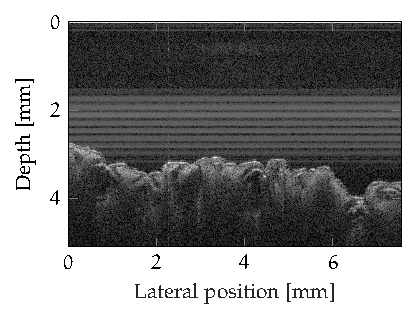
\includegraphics[width=0.75\linewidth]{gfx/ch4/axsun/bande/dry-orange-peel}
%	\caption{B-scan of dry orange peel.}\label{fig:dry-orange-peel-bande}
%\end{figure}


%\begin{figure}[hbt]
%	\myfloatalign
%	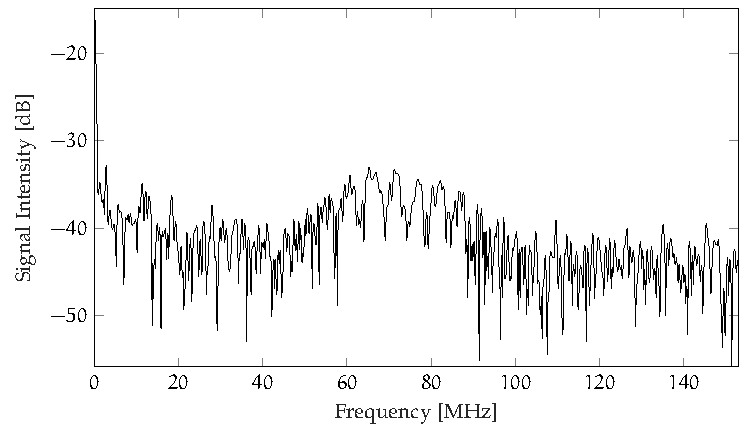
\includegraphics[width=\linewidth]{gfx/tikz/axsun/spurious-frequencies}
%	\caption{Spurious beat frequencies detected by the Exalos \ac{BPD}.}\label{fig:spurious-frequencies}
%\end{figure}



In these images a series of horizontal bands occupy the middle of the imaging range. The cause of this effect has not yet been determined, but it has been observed that placing a polarization controller after the reference arm reduces the visibility of these artifacts. 

This can be seen in the following images, representing:
\begin{itemize}
	\item a fresh orange peel (\autoref{fig:orange-peel}): the glans containing the natural oil are visible.
	
	\item a sliced cherry tomato (\autoref{fig:tomato-1}). Notice the highly scattering seeds and the reticular structure of the pulp;
	
	\item a strawberry (\autoref{fig:strawberry});
	
	\item an onion (\autoref{fig:red-onion-2});
	
	\item human fingernail (\autoref{fig:finger-gian}) and fingertip (\autoref{fig:finger-leo-2}): fingerprints, epidermis and dermis layers are all clearly recognizable.
	
	\item a piece of beef steak (\autoref{fig:steak}): \autoref{fig:beef-steak} represents the various layers of muscle of a lean part of the steak, while in \autoref{fig:fat-steak} a section of fat tissue is illustrated.
\end{itemize}

\begin{figure}[hbt]
	\centering
	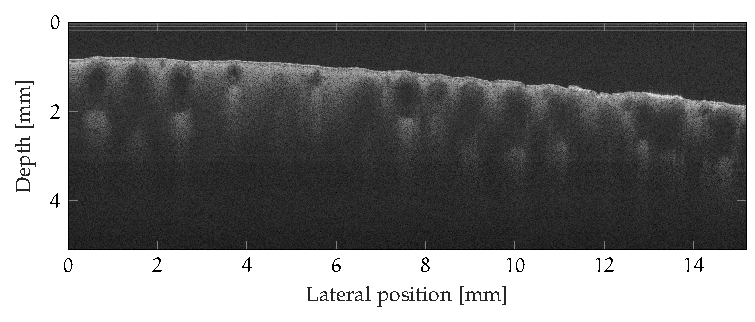
\includegraphics[width=0.9\linewidth]{gfx/ch4/axsun/no-bande/orange-peel}
	\caption{B-scan of an orange peel.}\label{fig:orange-peel}
\end{figure}

\begin{figure}[hbt]
	\centering
	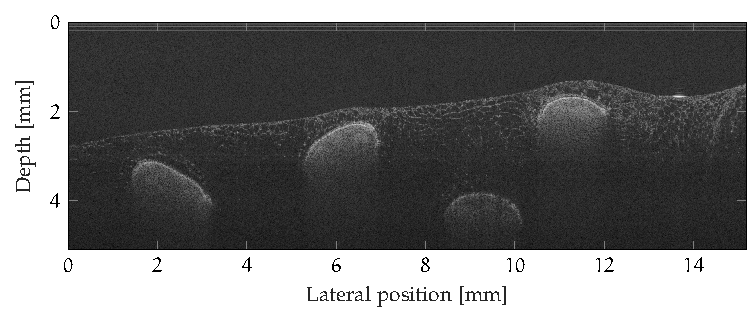
\includegraphics[width=0.9\linewidth]{gfx/ch4/axsun/no-bande/tomato-1}
	\caption{B-scan of a cherry tomato.}\label{fig:tomato-1}
\end{figure}

\begin{figure}[htb]
	\centering
	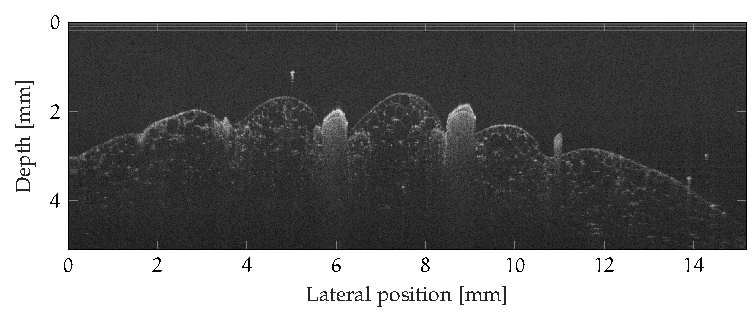
\includegraphics[width=0.9\linewidth]{gfx/ch4/axsun/no-bande/strawberry-1}
	\caption{B-scan of a strawberry.}\label{fig:strawberry}
\end{figure}	

\begin{figure}[htb]
	\centering
	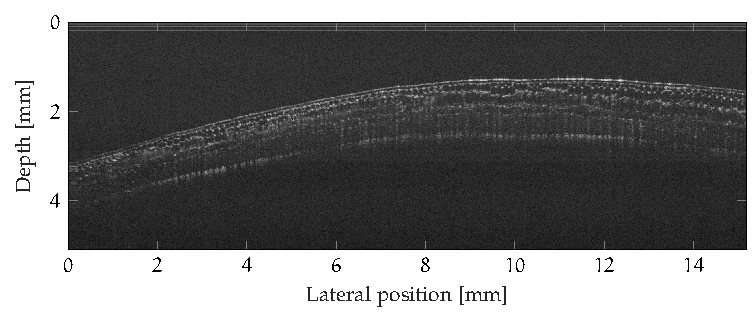
\includegraphics[width=0.9\linewidth]{gfx/ch4/axsun/no-bande/red-onion-2}
	\caption{B-scan of an onion.}\label{fig:red-onion-2}
\end{figure}

\begin{figure}[htb]
	\myfloatalign
	\subfloat[Human nail.]
	{\label{fig:finger-gian}
		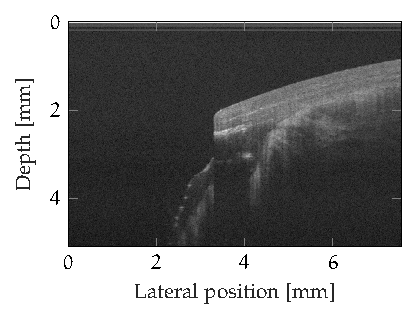
\includegraphics[width=.47\linewidth]{gfx/ch4/axsun/no-bande/finger-gian}} \quad
	\subfloat[Fingertip.]
	{\label{fig:finger-leo-2}
		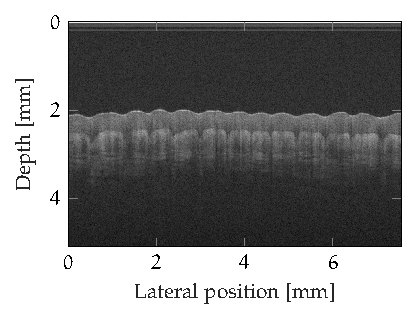
\includegraphics[width=.47\linewidth]{gfx/ch4/axsun/no-bande/finger-leo-2}} \\
	\caption{B-scans of a human finger.}\label{fig:human-finger}
\end{figure}


\begin{figure}[htb]
	\myfloatalign
	\subfloat[Lean tissue.]
	{\label{fig:beef-steak}
		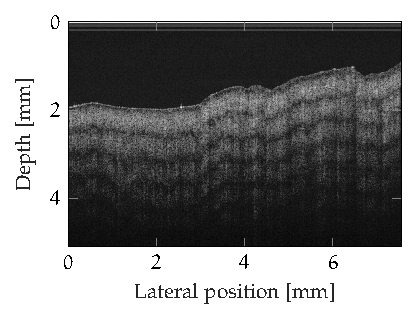
\includegraphics[width=.47\linewidth]{gfx/ch4/axsun/no-bande/steak-2}} \quad
	\subfloat[Fat tissue.]
	{\label{fig:fat-steak}
		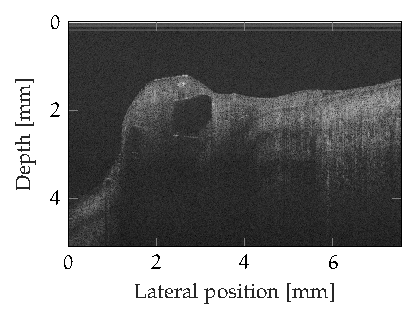
\includegraphics[width=.47\linewidth]{gfx/ch4/axsun/no-bande/steak-fat-2}} \\
	\caption{B-scans of a beef steak.}\label{fig:steak}
\end{figure}

%%%%%%%%%%%%%%%%%%%%%

%\begin{figure}[hbt]
%	\centering
%	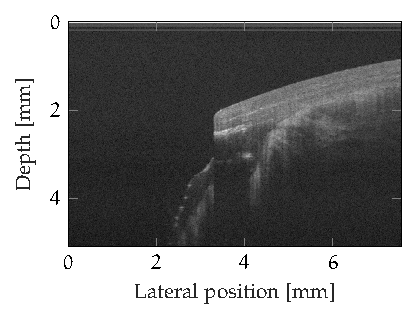
\includegraphics[width=0.8\linewidth]{gfx/ch4/axsun/no-bande/finger-gian}
%	\caption{B-scan of the Thorlabs test target.}\label{fig:finger-gian}
%\end{figure}
%
%
%\begin{figure}[hbt]
%	\centering
%	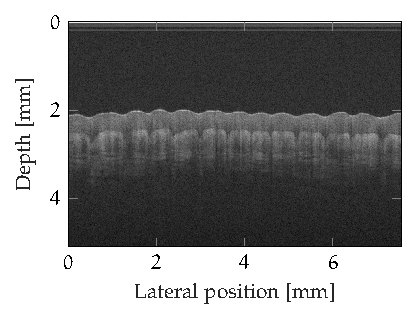
\includegraphics[width=0.8\linewidth]{gfx/ch4/axsun/no-bande/finger-leo-2}
%	\caption{B-scan of the Thorlabs test target.}\label{fig:finger-leo-2}
%\end{figure}

%%%%%%%%%%%%%%%%%%%%%

\clearpage
\subsection{SS-OCT at 1060 nm}
A second SS-OCT system working in the 1060 nm range and based on the design presented in this thesis was also tested. The setup is available in \autoref{fig:santec-setup}: using a fixed fiber reflector in the reference arm requires a \ac{VOA} to limit the power received by the BPD and a more complicated calibration of the sample arm. In fact, after measuring the length of the reference arm with a \ac{OFDR}, a fiber patch cord of the appropriate length was built by cutting and splicing two separate patch cords. 

Optical components such as scanning lens and collimators are equivalent to those introduced in \autoref{ch:setup}. The laser is instead a Santec HSL, capable of a selectable sweep rate and maximum imaging depth of $\sim 9$ mm. 


\begin{figure}[htb]
	\centering
	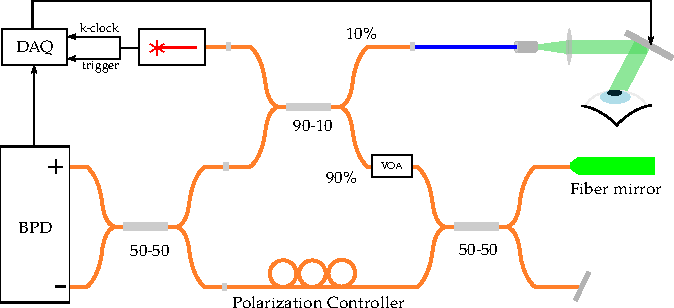
\includegraphics[width=\linewidth]{gfx/ch4//santec-setup}
	\caption{Setup of the SS-OCT system working in the 1060 nm range.}\label{fig:santec-setup}
\end{figure}

\subsubsection{B-scans}

Two B-scans acquired with this system are available in \autoref{fig:santec-bscans}: the juice vesicles of an orange slice are reported \autoref{fig:santec-orange}, while a scotch tape roll covering the entire imaging range is visible in \autoref{fig:santec-tape}. 

\begin{figure}[htb]
	\myfloatalign
	\subfloat[Orange slice.]
	{\label{fig:santec-orange}
		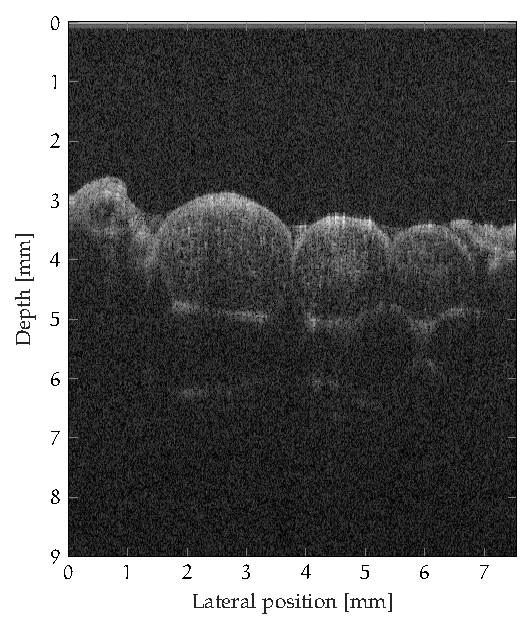
\includegraphics[width=.47\linewidth]{gfx/ch4/santec/orange-2}} \quad
	\subfloat[Scotch tape.]
	{\label{fig:santec-tape}
		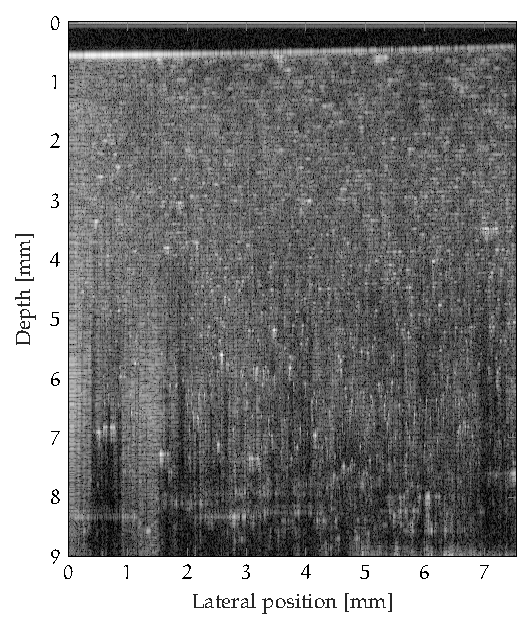
\includegraphics[width=.47\linewidth]{gfx/ch4/santec/tape-3}} \\
	\caption{B-scans acquired with the 1060 nm system.}\label{fig:santec-bscans}
\end{figure}

By changing the state of polarization of the field reflected by the reference arm with the polarization controller, some birefringence-induced effects can be observed. An example is provided in \autoref{fig:santec-tape-birefringence}, where B-scans of a roll of scotch tape are acquired with the polarization controller in two different positions. We can see that in the right image a black band appears in the middle of the tape. The birefringence of the material at that specific depth causes a reflection with a state of polarization that is almost-orthogonal to that imposed by the polarization controller, resulting in a lower intensity interference. 

\begin{figure}[htb]
	\myfloatalign
	\subfloat[]
	{\label{fig:tape-no-birefringence}
		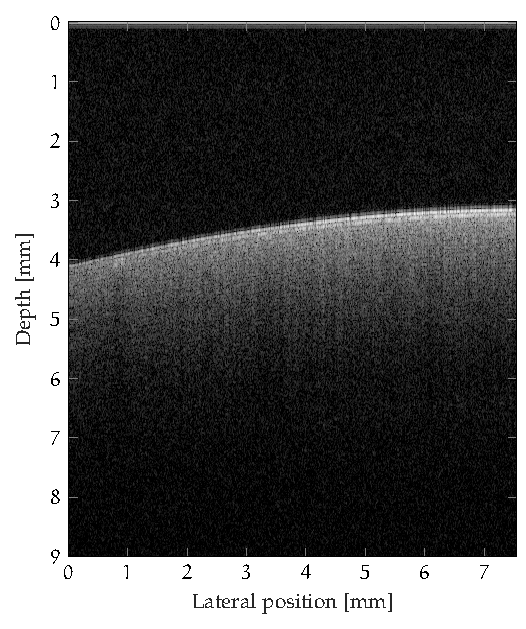
\includegraphics[width=.47\linewidth]{gfx/ch4/santec/tape-no-birefringence}} \quad
	\subfloat[]
	{\label{fig:tape-birefringence}
		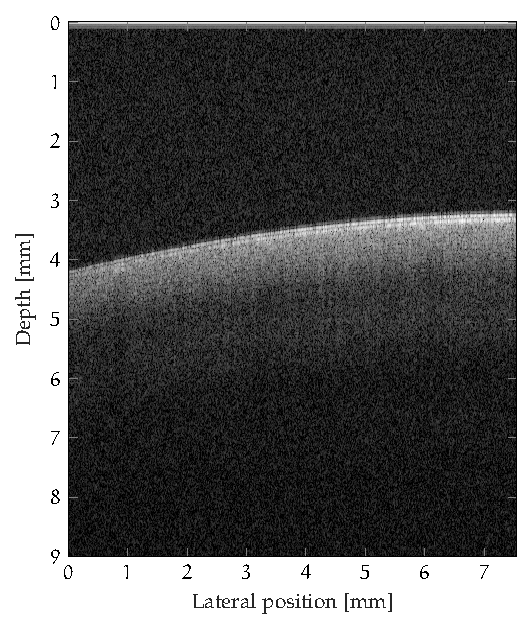
\includegraphics[width=.47\linewidth]{gfx/ch4/santec/tape-birefringence}} \\
	\caption{Birefringence effect on the B-scan of a scotch tape roll.}\label{fig:santec-tape-birefringence}
\end{figure}
\FloatBarrier
\subsubsection{Imaging of dynamic samples}
In order to test the OCT software with a dynamic sample, vinegar was poured in a microscope slide containing a small quantity of sodium bicarbonate. The two components cause a small reaction resulting in the generation of foam and bubbles. 
\begin{figure}[htb]
	\centering
	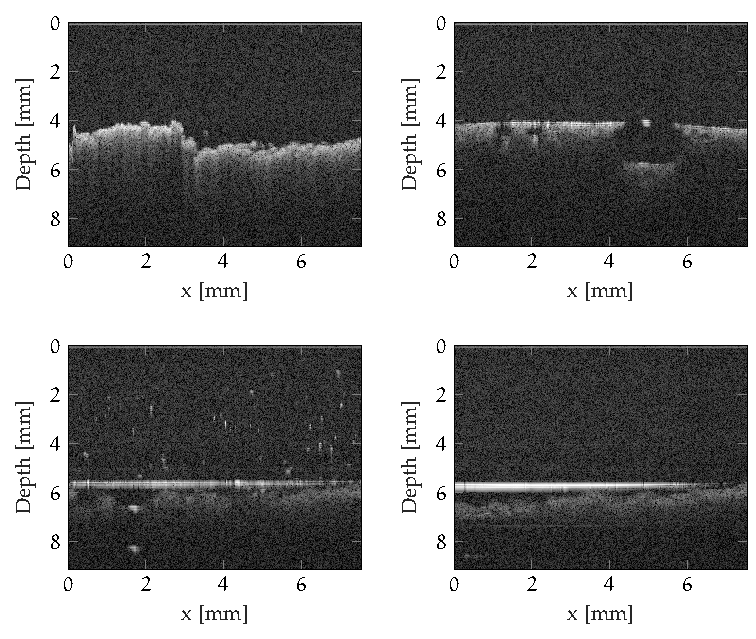
\includegraphics[width=\linewidth]{gfx/ch4/santec/aceto}
	\caption[]{Reaction between sodium bicarbonate and vinegar.}\label{fig:aceto}
\end{figure}
A few frames of the acquired video are presented in \autoref{fig:aceto}: in the top left the bicarbonate is in its resting state; after pouring vinegar with a syringe, bubbles start forming (top right); a few seconds later the reaction slows down and the bicarbonate begins to settle on the bottom surface (bottom left) while a few particles jump out of the slide; finally the reaction halts (bottom right) with the particles completely sedimented on the bottom of the slide. 

\clearpage
\subsection{En-face images}
\label{sub:enface}
In the introductory chapters of this thesis the concept of \emph{en-face} images was explained: a frontal view of the imaged sample can be reconstructed from a series of B-scans acquired at slightly different positions on the transverse plane. 

Usually, each pixel of the \emph{en-face} image is obtained from the corresponding A-scan by summing its values: in this way parts of the sample that are beneath the surface are represented in the frontal view. A second method that can be used to build the image is selecting the maximum value of each A-scan. Since the reflection coming from the surface of the sample is often the most intense, the resulting image is essentially a magnified version of the sample. 

The two processing methods are compared in the following figures, where the images on the left are generated with the \emph{max} method, while those on the right are the result of the traditional \emph{sum} method. 

\begin{figure}[H]
	\myfloatalign
	\subfloat[]
	{\label{fig:orange-peel-surf-photo}
		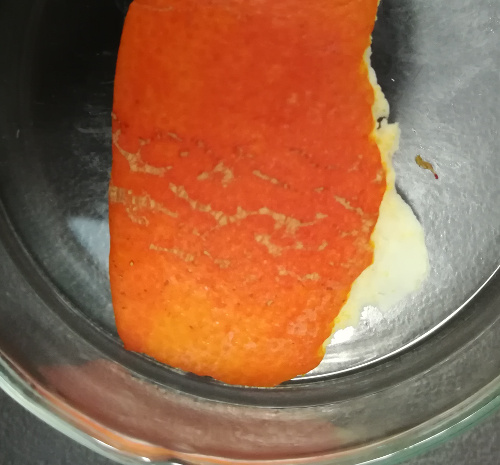
\includegraphics[width=0.4\linewidth]{gfx/ch4/orange-peel}}\\
	\subfloat[]
	{\label{fig:orange-peel-surf-enface}
	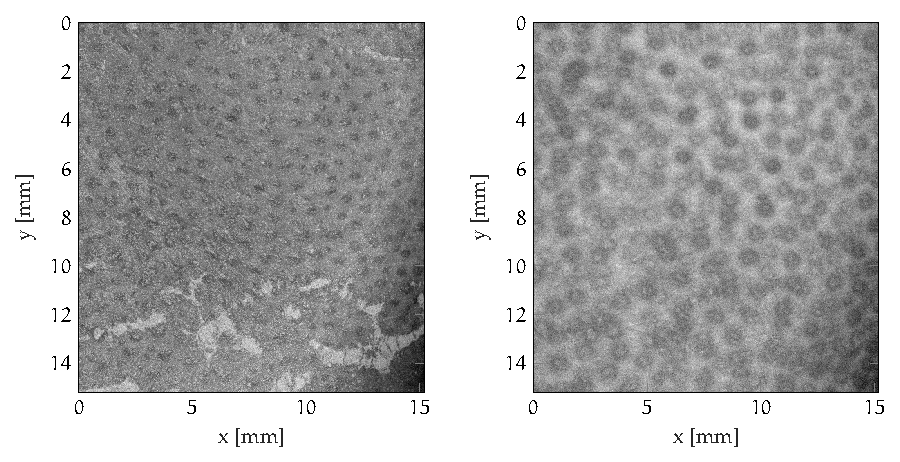
\includegraphics[width=\linewidth]{gfx/ch4/axsun/enface/orange-peel-surf}}
	\caption{\emph{En-face} view of an orange peel.}\label{fig:orange-peel-surf}
\end{figure}
The difference between the two procedures is clearly observable in \autoref{fig:orange-peel-surf}, where the \emph{en-face} view of an orange peel is presented. In the left image we can see the top portion of the glans and a defect mark on the lower part of the picture, while on the right the glans are entirely represented and the defect is not visible. 

\begin{figure}[H]
	\myfloatalign
	\subfloat[]
	{\label{fig:tomato-surf-photo}
		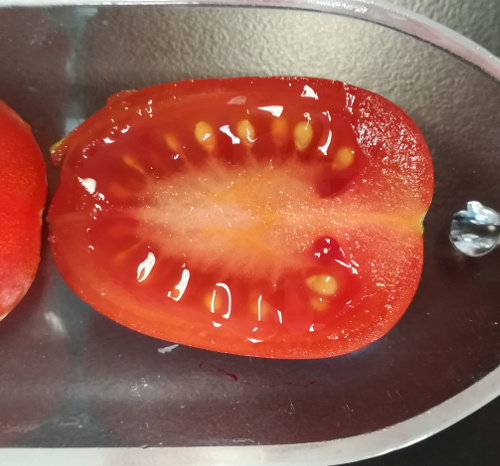
\includegraphics[width=0.4\linewidth]{gfx/ch4/tomato}}\\
	\subfloat[]
	{\label{fig:orange-peel-enface}
		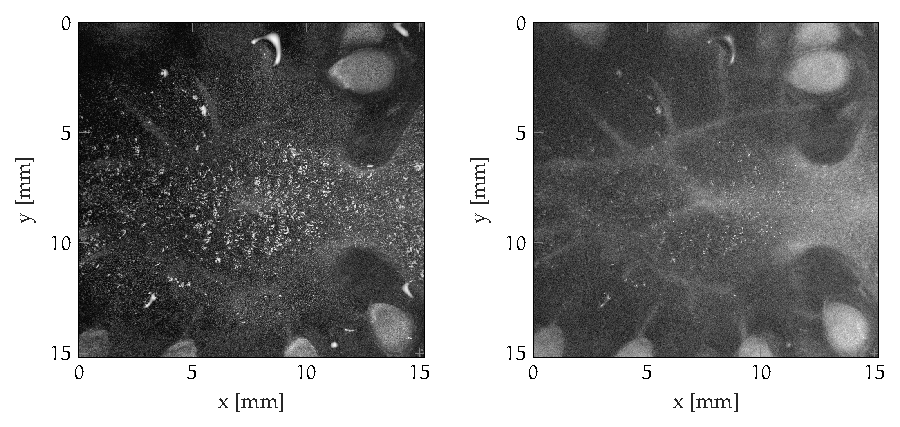
\includegraphics[width=\linewidth]{gfx/ch4/axsun/enface/tomato-surf}}
	\caption{\emph{En-face} view of sliced cherry tomato.}\label{fig:tomato-surf}
\end{figure}

A similar effect is observable in the \emph{en-face} projections of a cherry tomato presented in \autoref{fig:tomato-surf}, where the veins located underneath the top surface are only detected by the \emph{sum} method.

Other examples are available in \autoref{fig:enface-examples} which includes, from top to bottom: a sliced onion, a human fingertip, a strawberry, and an orange slice. As can be seen from these figures, the \emph{sum} method generally produces smoother images. 

\begin{figure}[hbt]
	\myfloatalign
%	\subfloat[]
	{\label{fig:fig:onion-surf}
		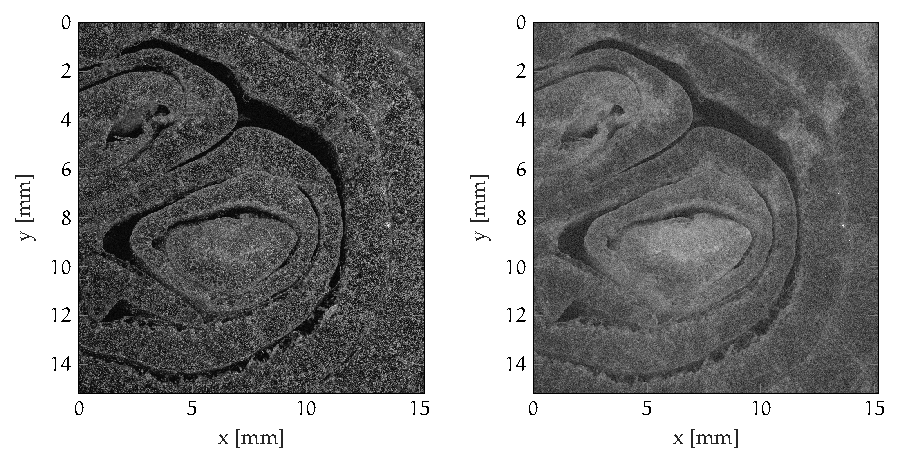
\includegraphics[width=1\linewidth]{gfx/ch4/axsun/enface/onion-surf}}\\
%	\subfloat[]
	{\label{fig:enface-fingerprint}
		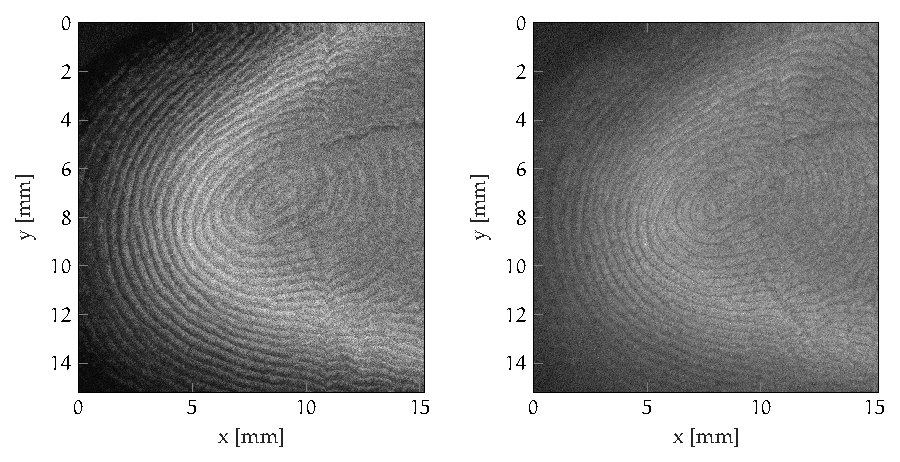
\includegraphics[width=1\linewidth]{gfx/ch4/santec/fingervolume-2}}\\
%	\subfloat[]
	{\label{fig:strawberry-surf}
		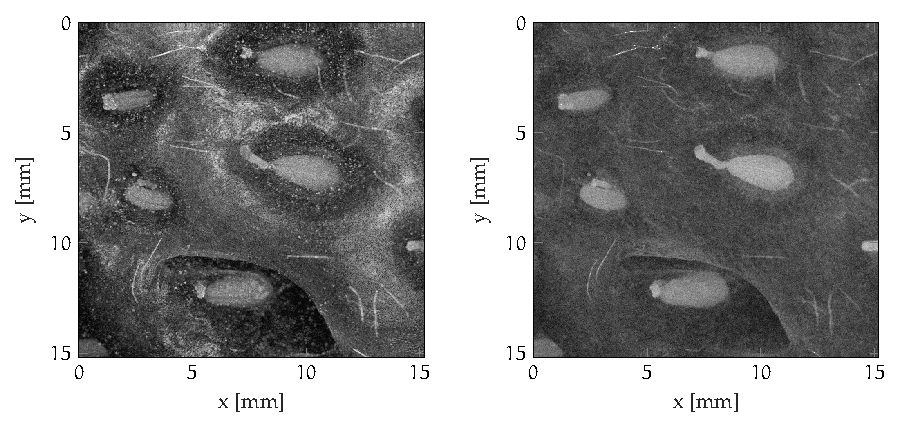
\includegraphics[width=1\linewidth]{gfx/ch4/axsun/enface/strawberry-surf}}\\
%	\subfloat[]
	{\label{fig:fig:orange-surf}
		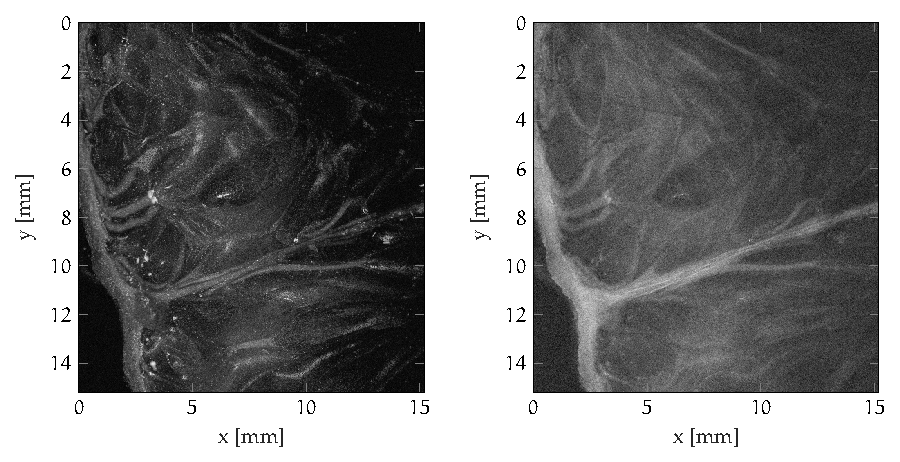
\includegraphics[width=1\linewidth]{gfx/ch4/axsun/enface/orange-surf}}\\
	\caption{\emph{En-face} images generated using the \emph{max} (left) and \emph{sum} (right) methods. From top to bottom: sliced onion, human fingertip, strawberry, orange slice.}\label{fig:enface-examples}
\end{figure}
%
%\begin{figure}[hbt]
%	\centering
%	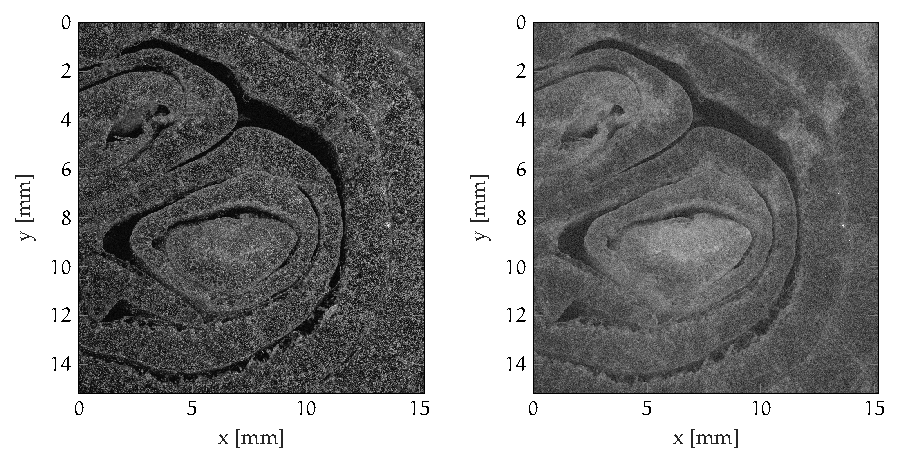
\includegraphics[width=\linewidth]{gfx/ch4/axsun/enface/onion-surf}
%	\caption{\emph{En-face} view of a sliced onion.}\label{fig:onion-surf}
%\end{figure}
%
%\begin{figure}[hbt]
%	\centering
%	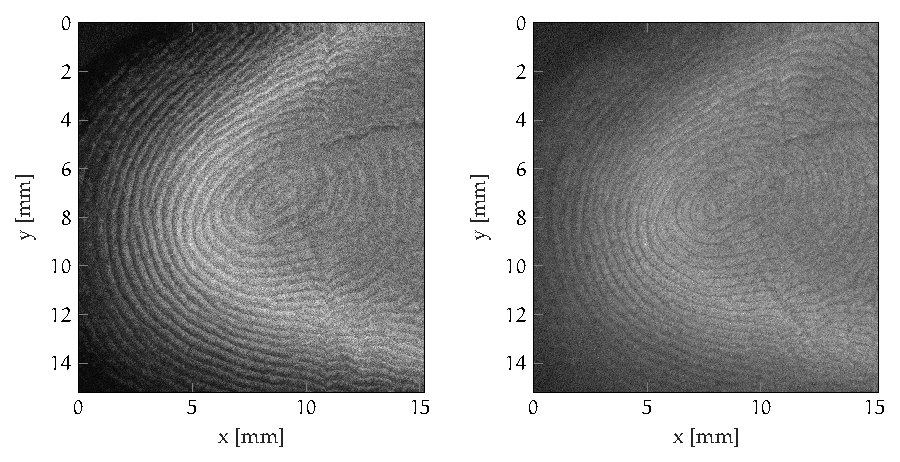
\includegraphics[width=\linewidth]{gfx/ch4/santec/fingervolume-2}
%	\caption{\emph{En-face} view of fingerprints.}\label{fig:enface-fingerprint}
%\end{figure}
%
%
%
%
%\begin{figure}[hbt]
%	\centering
%	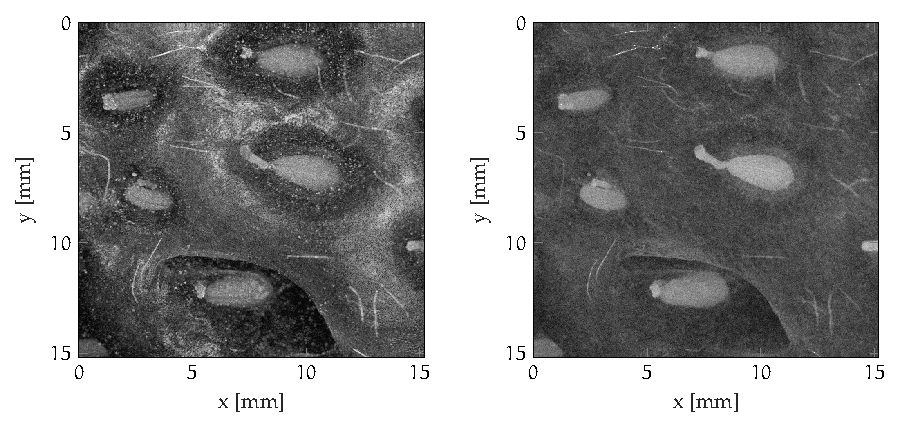
\includegraphics[width=\linewidth]{gfx/ch4/axsun/enface/strawberry-surf}
%	\caption{\emph{En-face} view of a strawberry.}\label{fig:strawberry-surf}
%\end{figure}
%
%\begin{figure}[hbt]
%	\centering
%	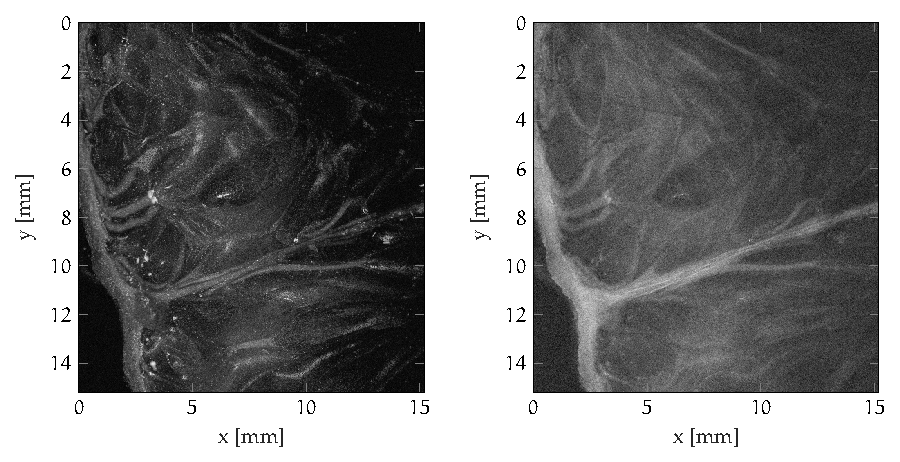
\includegraphics[width=\linewidth]{gfx/ch4/axsun/enface/orange-surf}
%	\caption{\emph{En-face} view of an orange slice.}\label{fig:orange-surf}
%\end{figure}


\FloatBarrier
\subsection{Measuring the transversal resolution}
The transversal resolution of the SS-OCT is experimentally determined by generating \emph{en-face} images of the Thorlabs resolution test target introduced in \autoref{sub:thickness-measurements}. The resolution of an imaging system is often specified in \emph{line pairs per millimiter} (lp/mm), whose value represents the smallest distance between two objects that can be registered by the system. The R1L1S1N test target is composed of five different patterns that will be presented in the following sections. Every acquisition has been performed by placing the top surface of the target on the focal plane of the scanning lens and with a sufficient number of points to guarantee a step size smaller than $1$ $\mu$m in each direction. 

\subsubsection{Grids}
This pattern consists in three grid patterns of different sizes: $10$ $\mu$m, $50$ $\mu$m and $100$ $\mu$m. The $10$ $\mu$m grid is a $20\times 20$ array with $1.5$ $\mu$m wide lines and a $10$ $\mu$m pitch in the $x$ and $y$ directions. The $50$ $\mu$m grid is a $20\times 20$ array with $1.5$ $\mu$m wide lines and a $50$ $\mu$m pitch in the $x$ and $y$ directions. The $100$ $\mu$m grid is a $20\times 20$ array with $5$ $\mu$m wide lines and a $100$ $\mu$m pitch in the $x$ and $y$ directions. 

The grid arrays are used to determine the distortion of a system, as the horizontal and vertical lines of the grid should be perpendicular to each other. A distorted image will show the lines as bent. The acquired image of this pattern is available in \autoref{fig:target-grid}: the $50$ and $100$ $\mu$m grids (center and right) are clearly visible and do not present any distortion. The $10$ $\mu$m is instead completely blurred, with the lines appearing as a unique block. The resolution of the system is then necessarily worse than $10$ $\mu$m. 

\begin{figure}[hbt]
	\centering
	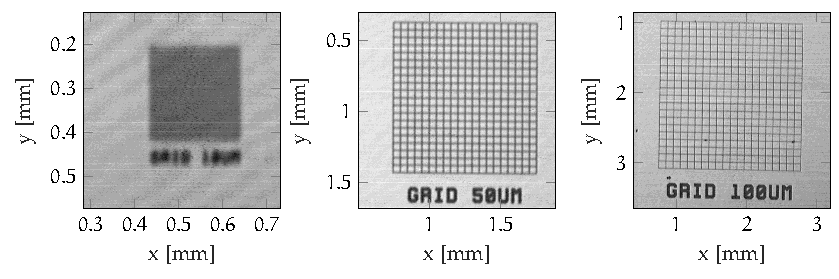
\includegraphics[width=\linewidth]{gfx/ch4/axsun/target/grid}
	\caption{\emph{En-face} projection of the grid pattern.}\label{fig:target-grid}
\end{figure}


\subsubsection{USAF 1951}
The USAF 1951 is a resolution test pattern conforming to the MIL-STD-150A standard set by the United States Air Force in 1951. The pattern is composed by six groups of six elements, each consisting in horizontal and vertical line pairs of different sizes. The resolution in lp/mm is computed as
\begin{equation}\label{eq:usaf}
	\delta x,y = 2^{\text{Group} + \left(\frac{\text{Element} - 1}{6}\right)},
\end{equation}
where "Element" is the largest set of non-distinguishable horizontal and vertical lines and "Group" is the index of the group in which this element is contained. The central part of this pattern is acquired and illustrated in \autoref{fig:target-usaf}, where groups 4, 5, 6 and 7 are visible. Looking at elements 4, 5 and 6 of group 5, it appears that vertical lines are more easily distinguished than horizontal lines. In fact, the first element in which vertical lines are not distinguished is element 1 of group 6, while for horizontal lines it is element 6 of group 5. Using \autoref{eq:usaf}, the $x$ and $y$ resolutions are
\begin{align}
	&\delta x \approx 64 \text{ lp/mm} \implies 15.6\,\mu\text{m} \\
	&\delta y \approx 57 \text{ lp/mm} \implies 17.5\,\mu\text{m},
\end{align}
which are a considerable improvement with respect to the theoretical value of $22.5$ $\mu$m computed in \autoref{eq:transversal-resolution-theory}. 

\begin{figure}[hbt]
	\centering
	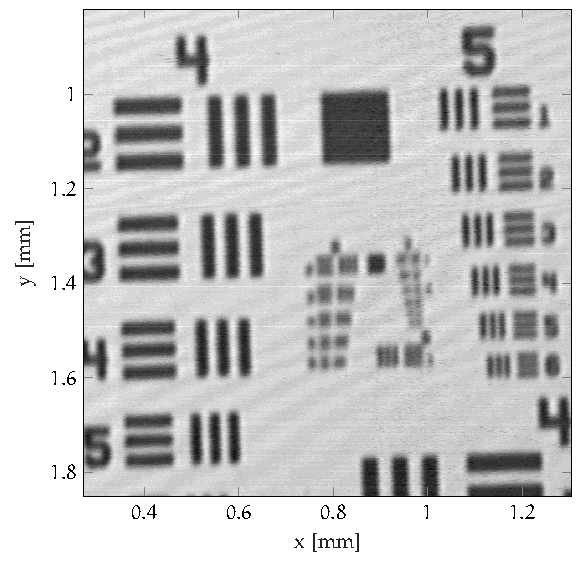
\includegraphics[width=0.6\linewidth]{gfx/ch4/axsun/target/usaf}
	\caption{\emph{En-face} projection of the USAF 1951 test target.}\label{fig:target-usaf}
\end{figure}

\subsubsection{Ronchi rulings}
Ronchi rulings are a set of parallel bars with widths that are equal to the distance between them. This pattern consists in thirteen 1 mm square Ronchi gratings with variable widths capable of measuring resolutions from 30 lp/mm up to 150 lp/mm. \autoref{fig:target-ronchi} all the thirteen gratings are visible. 

\begin{figure}[hbt]
	\centering
	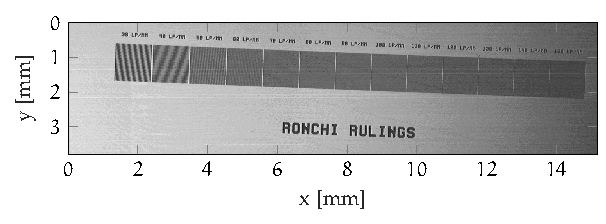
\includegraphics[width=1\linewidth]{gfx/ch4/axsun/target/ronchi-full}
	\caption{\emph{En-face} projection of variable frequency Ronchi rulings.}\label{fig:target-ronchi}
\end{figure}




A detailed view of the 60, 70 and 80 lp/mm rulings is instead presented in \autoref{fig:target-ronchi-detail}, where we can see that the vertical lines are distinguishable in the first two gratings but not in the last. Unlike with the USAF target, the resolution in this case is determined by the last grating that the system is able to resolve, resulting in
\begin{equation}
\delta x \approx 70 \text{ lp/mm} \implies 14.3\, \mu\text{m}
\end{equation}


\begin{figure}[hbt]
	\centering
	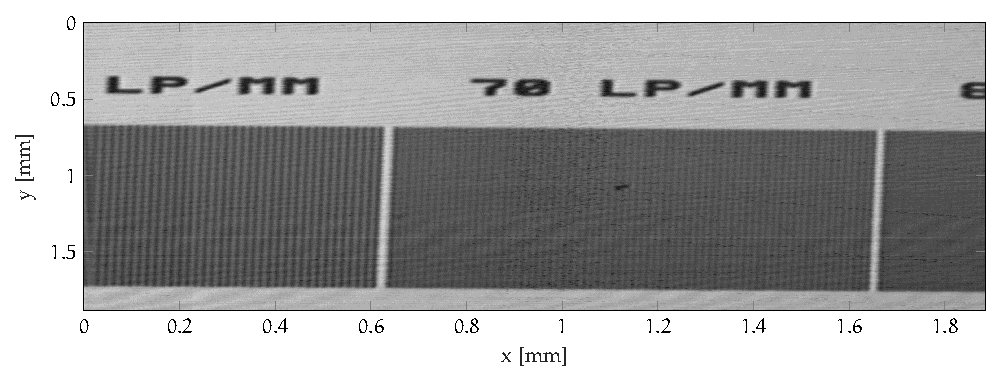
\includegraphics[width=1\linewidth]{gfx/ch4/axsun/target/ronchi-detail}
	\caption{\emph{En-face} projection of the 60, 70 and 80 lp/mm Ronchi gratings.}\label{fig:target-ronchi-detail}
\end{figure}

\subsubsection{Star Sector}
Sector star targets, also known as Siemens star targets, consist of a number of dark bars that increase in thickness as they radiate out from a shared center. Theoretically, the bars meet only at the exact middle point of the target, however this particular target has a blank center circle that cuts the bars off before they touch. Depending on the resolution of the optical system, the bars will appear to touch at some distance $r$ from the center. By measuring this distance, the user is able to define the resolution of the optical system with the following equation:
\begin{equation}
 \delta x  = \frac{1}{2r \sin(\theta / 2)},
\end{equation}
where $\theta$ is the number of degrees covered by one pair of light and dark bars, which for this particular target is equal to $\theta = 10^\circ$. To facilitate the reading of the radial distance, 10 clear concentric circles cut through the bars. The radii of these circles are: 50, 100, 150, 200, 250, 300, 350, 400, 450 and 500 $\mu$m. 

From \autoref{fig:target-star}, the bars appear to touch when reaching the second circle, meaning that $r = 100$ $\mu$m and resulting in

\begin{equation}
	\delta x \approx 57.4 \text{lp/mm} \implies 17.4\, \mu\text{m}
\end{equation}


\begin{figure}[hbt]
	\centering
	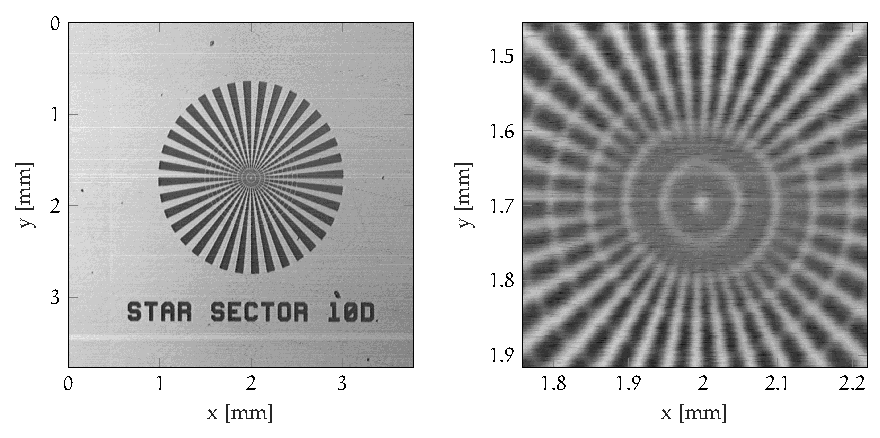
\includegraphics[width=1\linewidth]{gfx/ch4/axsun/target/star-sector}
	\caption{\emph{En-face} projection of the star sector pattern.}\label{fig:target-star}
\end{figure}

\subsubsection{Concentric circle}
This pattern consists in 10 concentric circles with cross lines in the center. The radius of each circle is a multiple of $100$ $\mu$m, starting from $100$ $\mu$ up to $1$ mm. The width of the arc line is instead $5$ $\mu$m. Concentric circles are mainly used to identify focusing errors, astigmatism and other aberrations introduced by the scanning system. 

\begin{figure}[hbt]
	\centering
	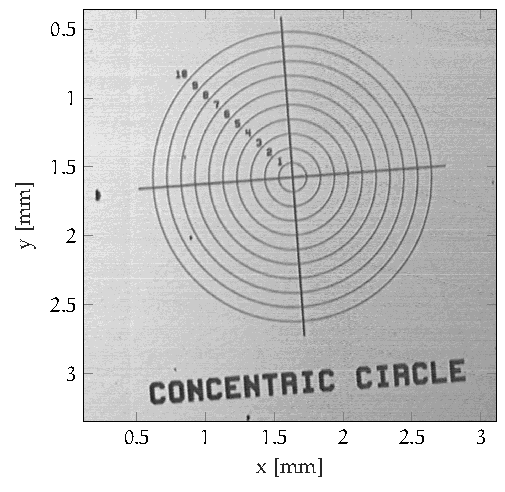
\includegraphics[width=0.5\linewidth]{gfx/ch4/axsun/target/concentric-circles}
	\caption{\emph{En-face} projection of the concentric circles.}\label{fig:concentric-circles}
\end{figure}

From \autoref{fig:concentric-circles} no apparent distortion is visible, suggesting a correct setup of the focusing optics. 



%\begin{figure}[bth]
%	\myfloatalign
%	\subfloat[Asia personas duo.]
%	{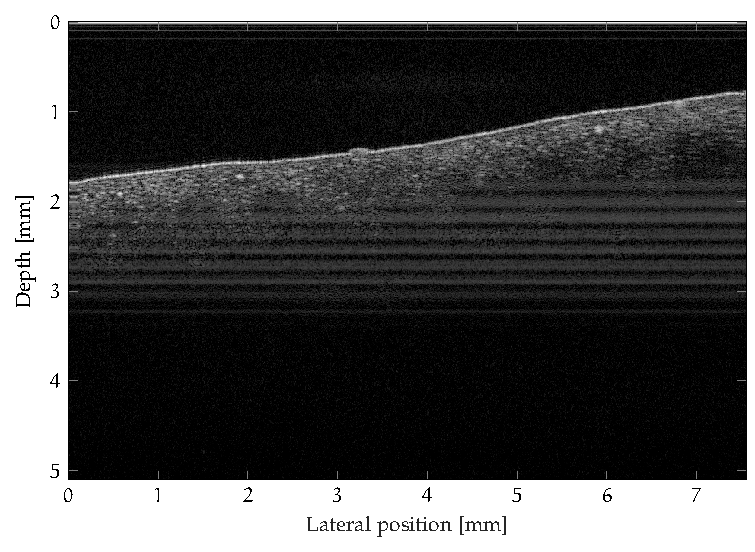
\includegraphics[width=.45\linewidth]{gfx/tikz/axsun/banana-peel}} \quad
%	\subfloat[Pan ma signo.]
%	{\label{fig:banan-peel}
%		\includegraphics[width=.45\linewidth]{gfx/tikz/axsun/tape}} \\
%	\subfloat[Methodicamente o uno.]
%	{\includegraphics[width=.45\linewidth]{gfx/tikz/axsun/nastro}} \quad
%	\subfloat[Titulo debitas.]
%	{\includegraphics[width=.45\linewidth]{gfx/tikz/axsun/spugna-1}}
%	\caption{Tu duo titulo debitas latente.}\label{fig:example}
%\end{figure}


\FloatBarrier
\subsection{Volumetric Data}
The last type of data that can be acquired with a OCT system is volumetric data. Each volume, or C-scan, is composed by a series of B-scans acquired at different positions on the sample. Unlike B-scans and \emph{en-face} projections, 3D data requires complex and efficient algorithms for a correct visualization. For this purpose, a C++ OpenGL application implementing a basic frame-based volumetric algorithm was developed.


 3D data is stored in a 3D texture object on the GPU, which will then compute a series of slices that cut through the texture perpendicular to the viewing direction (\autoref{fig:volume-slices}). Slices are then blended together using a blending equation and displayed on screen. Each time the viewing direction changes the slices have to be recomputed. 
  
 \begin{figure}[hbt]
 	\centering
 	\includegraphics[scale=0.5]{gfx/ch4/volume-slices}
 	\caption{Slicing of a 3D texture.}\label{fig:volume-slices}
 \end{figure}
 


In this implementation, B-scans are mapped from intensity values to RGBA space (Red, Green, Blue, Alpha) with a linear mapping, meaning that low intensity pixels will have a small Alpha value, making them more transparent. Advanced transfer functions can be implemented depending on the particular data that has to be visualized in order to use different colors for each material or structure in the sample. 

The application can also slice the texture along three orthogonal axes to obtain an equivalent B-scan for each direction. An example of these slices can be seen in the top portion of \autoref{fig:target-3d} along with the volumetric rendering of the USAF 1951 target. 

Other examples of C-scan rendering are available in \autoref{fig:3d-volumes}, where the same datasets used to compute \emph{en-face} projections in \autoref{sub:enface} are visualized. 

	\begin{figure}[hbt]
		\centering
		\includegraphics[width=0.92\linewidth,height=0.8\linewidth]{gfx/3d/target}
		\caption[]{Volume rendering and slicing of the USAF 1951 target.}\label{fig:target-3d}
	\end{figure}
%
%
%
%    \begin{figure}[hbt]
%        \centering
%        \includegraphics[width=0.9\linewidth]{gfx/3d/finger}
%        \caption[]{3D rendering of a human finger.}\label{fig:finger-3d}
%    \end{figure}
%
%	\begin{figure}[hbt]
%		\centering
%		\includegraphics[width=0.8\linewidth]{gfx/3d/strawberry}
%		\caption[]{3D rendering of a strawberry.}\label{fig:strawberry-3d}
%	\end{figure}
%
%	\begin{figure}[hbt]
%		\centering
%		\includegraphics[width=0.8\linewidth]{gfx/3d/onion}
%		\caption[]{3D rendering of an onion slice.}\label{fig:onion-3d}
%	\end{figure}
%
%	\begin{figure}[hbt]
%		\centering
%		\includegraphics[width=0.8\linewidth]{gfx/3d/orange}
%		\caption[]{3D rendering of an orange slice.}\label{fig:orange-3d}
%	\end{figure}

\begin{figure}[bth]
	\myfloatalign
	\subfloat[Human fingertip.]
	{\includegraphics[width=.45\linewidth]{gfx/3d/finger}} \quad
	\subfloat[Strawberry.]
	{\includegraphics[width=.45\linewidth]{gfx/3d/strawberry}} \\
	\subfloat[Onion.]
	{\includegraphics[width=.45\linewidth]{gfx/3d/onion}} \quad
	\subfloat[Orange.]
	{\includegraphics[width=.45\linewidth]{gfx/3d/orange}}
	\caption{Volume rendering of OCT data.}\label{fig:3d-volumes}
\end{figure}

    
